\documentclass[reprint,norsk,notitlepage]{revtex4-2}
\usepackage{amsmath}
\usepackage[mathletters]{ucs}
\usepackage[utf8x]{inputenc}
\usepackage[norsk]{babel}
\usepackage{esint}
\usepackage{physics,amssymb}
\usepackage{graphicx}
\usepackage{xcolor}
\usepackage[colorlinks]{hyperref}
\usepackage{cleveref}
\usepackage{listings}
\usepackage{subfig}
\usepackage{booktabs}
\usepackage{caption}
\usepackage{listings}

\hypersetup{
    colorlinks,
    linkcolor={red!50!black},
    citecolor={blue!50!black},
    urlcolor={blue!80!black}}

\lstset{inputpath=,
    backgroundcolor=\color{white!88!black},
    basicstyle={\ttfamily\scriptsize},
    commentstyle=\color{magenta},
    language=Python,
    morekeywords={True,False},
    tabsize=4,
    stringstyle=\color{green!55!black},
    frame=single,
    keywordstyle=\color{blue},
    showstringspaces=false,
    columns=fullflexible,
    keepspaces=true}

\begin{document}

\title{Lab Rapport - Solcellen}
\author{}
\affiliation{University of Oslo}
\date{\today}

\begin{abstract}
    Det ble gjennomført flere eksperimenter på solceller i forskjellige kretser og lysforhold for å undersøke hvordan solceller fungerer og hvordan de kan optimaliseres. Vi undersøkte hvordan solceller fungerer som halvlederdioder, hvordan de kan kobles i serie og parallel for å oppnå høyere spenning og strøm, og hvordan de oppfører seg i delvis skygge. Vi fant at solceller fungerer som halvlederdioder, og at de kan kobles i serie og parallel for å oppnå høyere spenning og strøm. Vi fant også at solceller oppfører seg annerledes i delvis skygge. Resultatene tilsier at solceller er svært sensitive for lysforhold og at for å optimaliseres må en ta hensyn til sitt unike miljø er en ønsker å bruke solcellene. 
\end{abstract}

\maketitle

\section{Introduksjon} \label{sec: introduction}
Solcellen er et viktig verktøy innen grønn energi som lar oss gjøre om sollys til elektrisk energi. De kan skaleres ned til å passe på en kalkulator eller skaleres opp til å dekke store "solcelle gårder". I motsetning til andre energi kilder som vann, olje eller kjernekraft, er solceller utsatt for ekstremt varierende forhold. Solceller er derfor et viktig verktøy å studere for å kunne utvikle mer effektive solceller som kan brukes i flere miljøer. Vi skal i denne rapporten utsette en solcelle for flere forhold og se hvordan vi kan optimalisere dets effektivitet. Eksperimentene vi skal gjennomføre består av fire deler.\newline

\paragraph*{1. Solcellen som halvleder diode}\mbox{}\\
Her undersøker vi strøm-spenning karakteristikken til solcellen. Vi måler strømmen ved forskjellige spenninger og analyserer resultatene. Dette skal gjøres både i lys og i mørke for å se hvordan denne kurven vil endre seg.
\begin{figure}[h!]
  \centering
  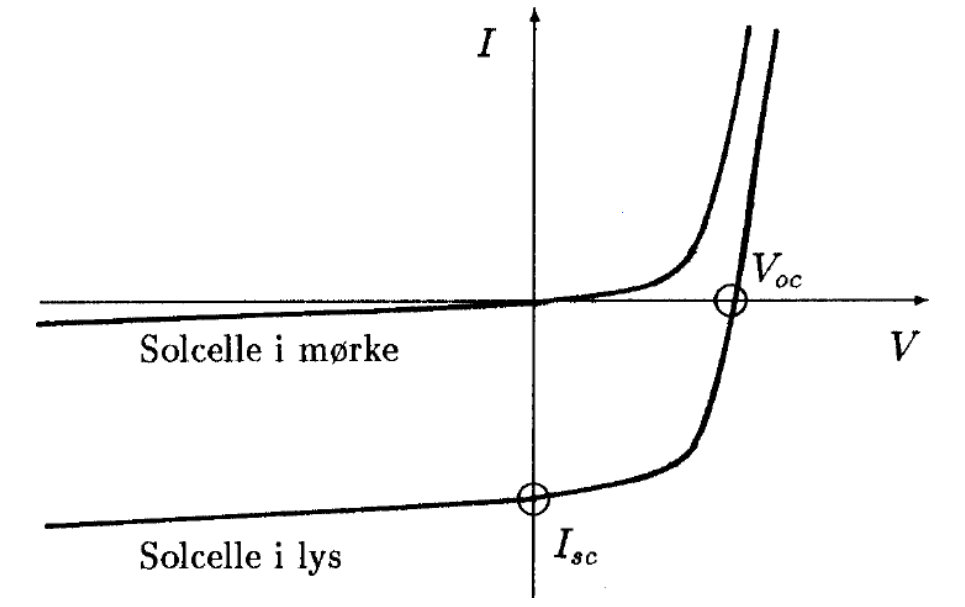
\includegraphics[width = 0.4\textwidth]{SS_kurve.png}
  \caption{Typisk strøm-spenning karakteristikk for en solcelle med og uten lys}
  \label{fig: SS_kurve}
\end{figure}

\paragraph*{2. Solcellens optimale belastning}\mbox{}\\
Avhengig av hva solcellen skal brukes til kan det være lønnsomt med høy strøm eller spenning. I denne delen er målet å finne maksimal strøm og spenning vi kan få ut av den, samt dets effekt.\newline

\paragraph*{3. Kombinasjon av enkeltsolceller til et solcellepanel}\mbox{}\\
Ved å koble solceller i serie vil vi kunne oppnå høyere spenning. I parallel, høyere strøm. Dette har både positive og negative sider vi skal utforske ved å koble sammen to solceller. Dette vil gi oss en bedre forståelse av hvordan vi kan optimalisere solcellepaneler for maksimal effekt.\newline
  
\paragraph*{4. Ikke-uniform belysning}\mbox{}\\
Til slutt skal vi gjenta forrige eksperiment for se hvordan delvis skygge påvirker de tidligere resultatene. Som tidligere nevnt er solceller ofte utsatt for veldig varierende forhold. Montert på en hytte kan solcellene oppleve delvis skygge fra trær, skygge, eller opphopning av skitt. Dette må vi ta med i betraktning når vi skal lage det mest effektive panelet mulig. 


\section{Teori} \label{sec: theory}
\subsection{Kretser}
Forholdet mellom strøm $I$, spenning $V$ og motstand $R$ er beskrevet i Ohms lov: 
\begin{equation}\label{eq: Ohms lov}
  V = IR
\end{equation}
Effekten $P$ til en krets, er mengden energi produsert per tidsenhet og er beskrevet på følgende måte
\begin{equation}\label{eq: Effekt}
  P = IV
\end{equation}

\section{Eksperimentelt} \label{sec: method}
\subsection{Solcellen som halvlederdiode}
\begin{figure}[h!]
    \centering
    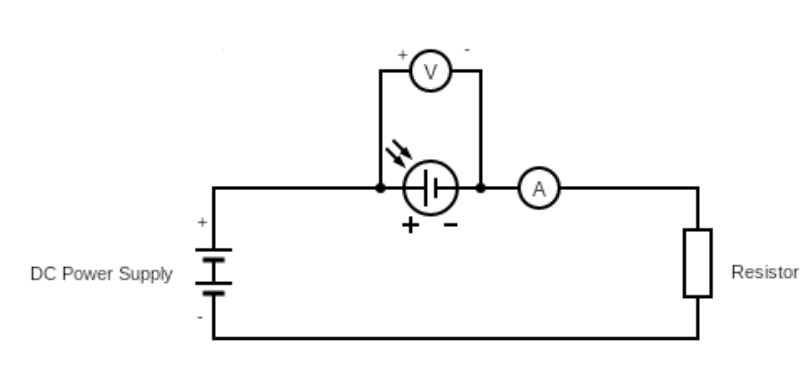
\includegraphics[width = 0.4\textwidth]{Oppsett_1.png}
    \caption{Oppsett av krets}
    \label{fig: Oppgave 1}
\end{figure}
I dette eksperimentet koblet i solcellen i en krets som illustrert i \cref{fig: Oppgave 1}. Vi målte strømmen $I$ ved forskjellige spenninger $V$ i et intervall som viste den forventede, eksponentielle veksten. Motstanden $R$ var på 10 Ohm. Strømmen økte veldig hurtig ved høyere spenning så vi hadde mindre økning i spenning når strømmen økte raskt for å observere denne endringen. Gjennom hele forsøket var solcellen dekt til for å ta opp minimalt med lys. Resultatene ble notert og plottet. 
\newpage

\begin{figure}[h!]
  \centering
  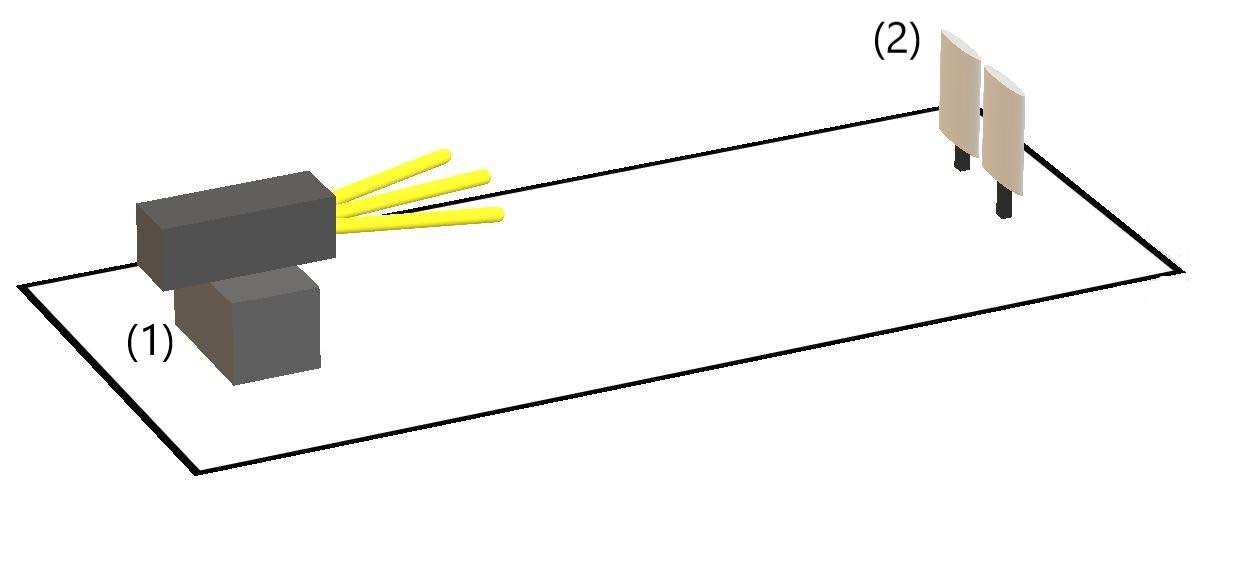
\includegraphics[width = .4\textwidth]{Opsett.jpg}
  \caption{Oppsett av solceller og lyskilde}
  \label{fig: Opsett}
\end{figure}


Vi setter opp kretsen som i \cref{fig: Oppgave 1}, men uten spenningskilden og motstand. Solcellene plasseres 60 cm unna en lyskilde og opprettholder jevn belysning som illustrert i \cref{fig: Opsett}. Begge solcellene er satt opp, men bare den ene er koblet til kretsen. Dette er gjort for å få sammenlignbare resultater med senere eksperimenter. Får å undersøke maksimal effekt gitt ved \cref{eq: Effekt} måler vi strøm og spenning ved varierende motstand $R ∈ [0.2, 10]$ Ohm. Resultatene blir plottet og analysert.

\subsection{Kombinasjon av enkeltsolceller til et solcellepanel}
\begin{figure}[h!]
  \centering
  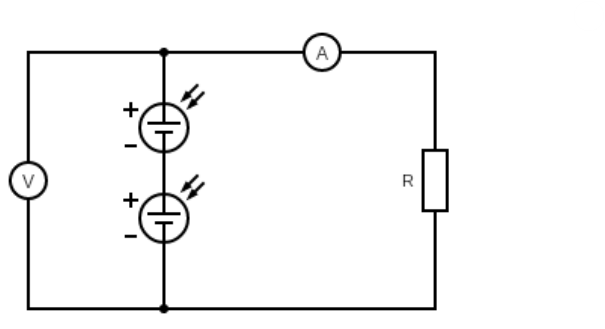
\includegraphics[width = .4\textwidth]{Solcelle_ser.png}
  \caption{To solceller koblet i serie}
  \label{fig: 3_ser}
\end{figure}

\begin{figure}[h!]
  \centering
  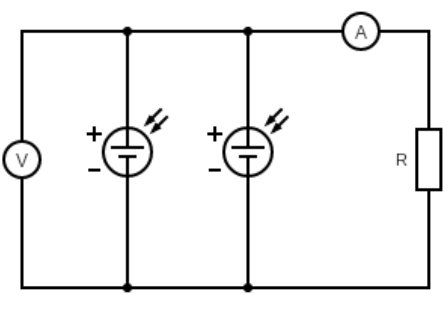
\includegraphics[width = .4\textwidth]{Solcelle_par.png}
  \caption{To solceller koblet i parallel}
  \label{fig: 3_par}
\end{figure}


Vi begynte først med å sette opp de to solcellene i serie som illustrert i \cref{fig: 3_ser}. Vi måler både strøm og spenning i mens vi varierer motstanden i samme intervall som i forrige eksperiment. 
Videre setter vi opp solcellene i parallel som illustrert i \cref{fig: 3_par}, og gjentar målingene. Resultatene blir plottet og analysert. 


\subsection{Ikke-uniform belysning}
I dette eksperimentet gjentok vi fremgangsmåten fra forrige eksperiment, men vi la til en skygge foran den ene solcellen. 

\section{Resultater} \label{sec: results}
\subsection{Solcellen som halvlederdiode}
\begin{figure}[h!]
  \centering
  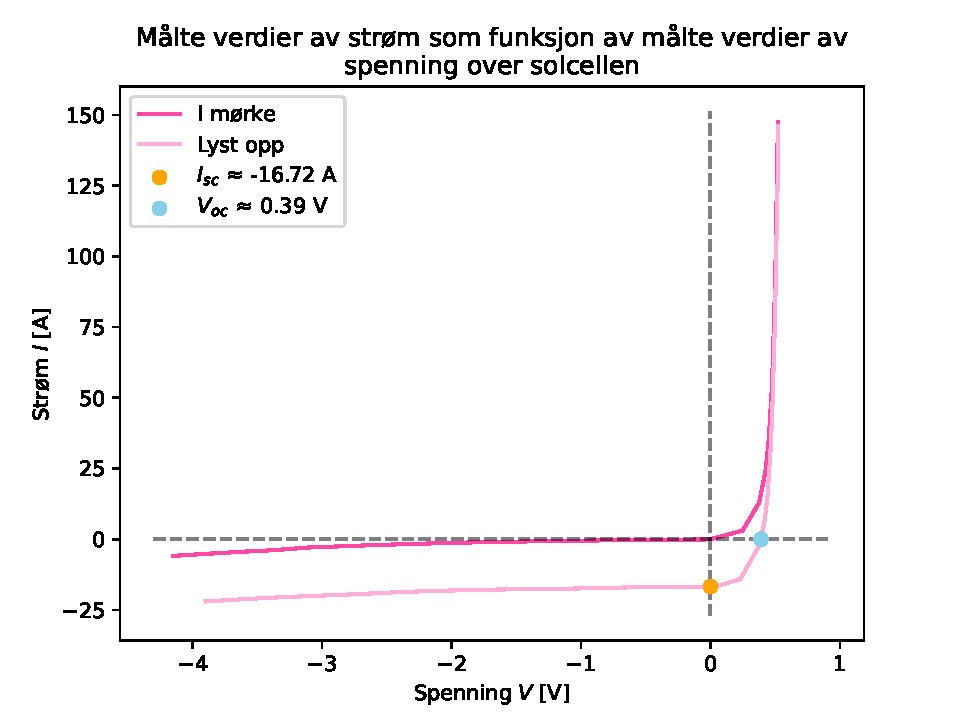
\includegraphics[width = .4\textwidth]{solcellen-oppg-1.pdf}
  \caption{Strøm-spenningskarakteristikk for en solcelle med og uten lys}
  \label{fig: strom-spenningskarakteristikk}
\end{figure}

Ved måling fant vi $I_{sc} = -16.7$A og $V_{oc} = 0.39$V som beskriver strømmen ved uendelig stor belastning og spenningen ved en kortsluttet krets. Verdiene kan også leses av i \cref{fig: strom-spenningskarakteristikk}.

\subsection{Solcellens optimale belastning}
\begin{figure}[h!]
  \centering
  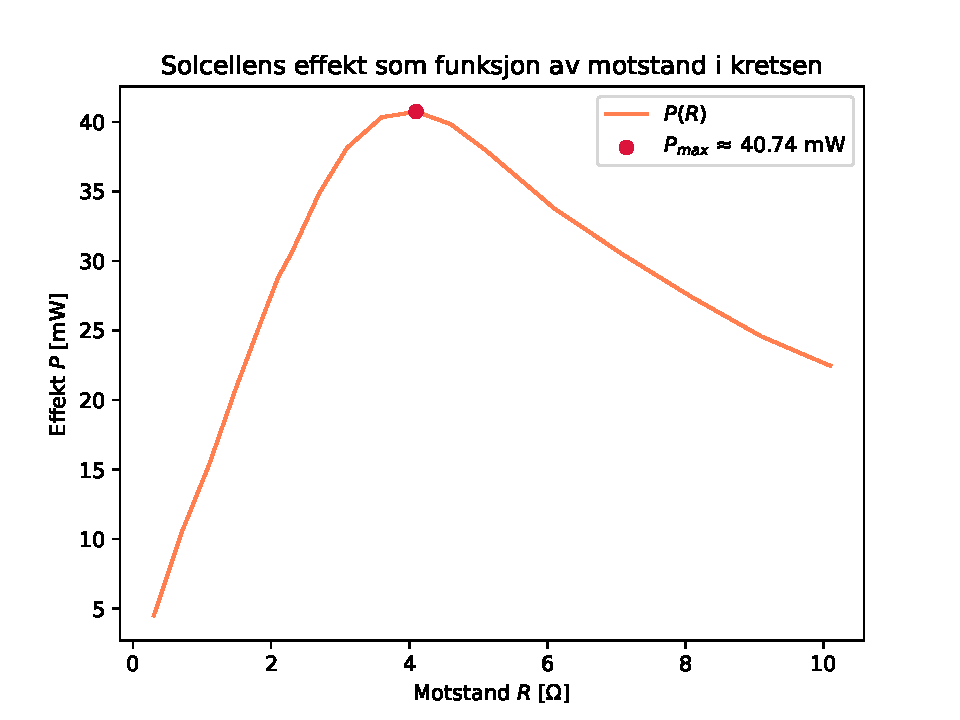
\includegraphics[width = .4\textwidth]{solcellen-oppg-2.pdf}
  \caption{Solcellens effekt som funksjon av motstand}
  \label{fig: effekt-motstand}
\end{figure}
Vi leser av toppunktet i \cref{fig: effekt-motstand} som gir $R_{opt} = 4.1$ Ohm og $P_{max} = 40.7$ mW.

\subsection{Kombinasjon av enkeltsolceller til et solcellepanel}
\begin{figure}[h!]
  \centering
  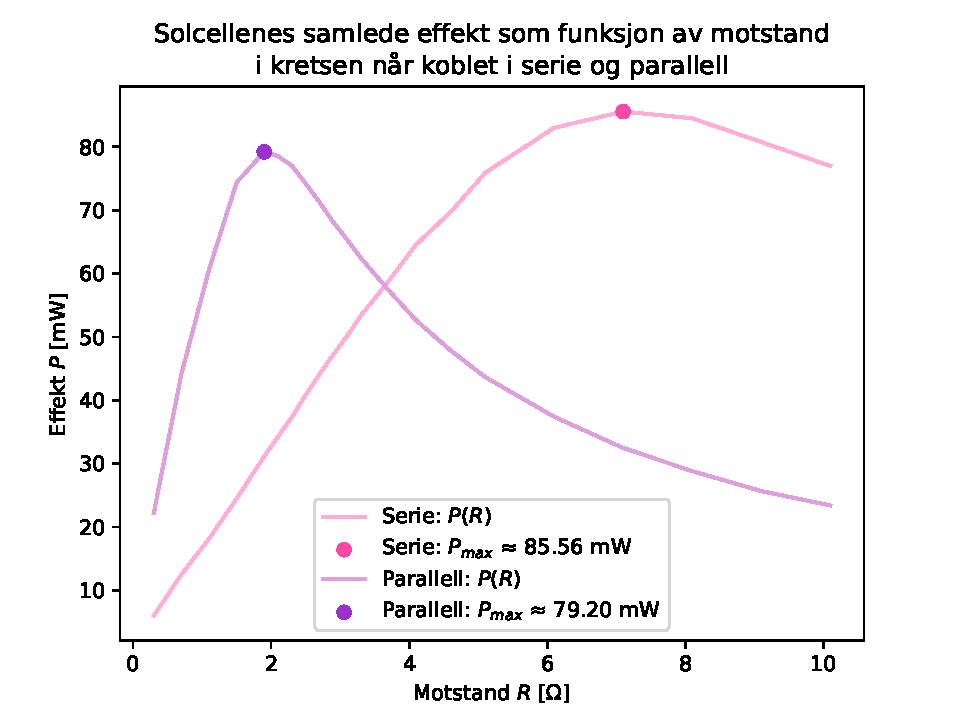
\includegraphics[width = .4\textwidth]{solcellen-oppg-3.pdf}
  \caption{Solcellens effekt som funksjon av motstand for to solceller koblet i serie og parallel}
  \label{fig: effekt-motstand-serie-parallel}
\end{figure}
Vi leser av toppunktene i \cref{fig: effekt-motstand-serie-parallel} som gir $R_{opt} = 7.1$ Ohm og $P_{max} = 85.6$ mW for solcellene koblet i serie og $R_{opt} = 1.9$ Ohm og $P_{max} = 79.2$ mW for solcellene koblet i parallel.
\subsection{Ikke-uniform belysning}
\begin{figure}[h!]
  \centering
  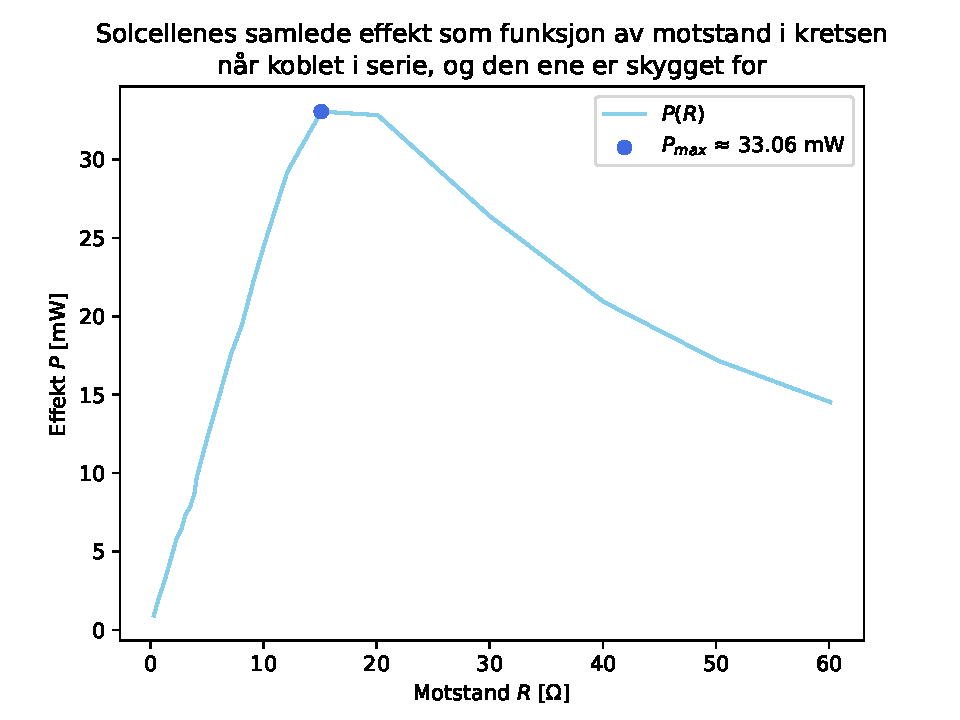
\includegraphics[width = .4\textwidth]{solcellen-oppg-4-serie.pdf}
  \caption{Solcellens effekt som funksjon av motstand for to solceller koblet i serie med skygge}
  \label{fig: effekt-motstand-serie-skygge}
\end{figure}

\begin{figure}[h!]
  \centering
  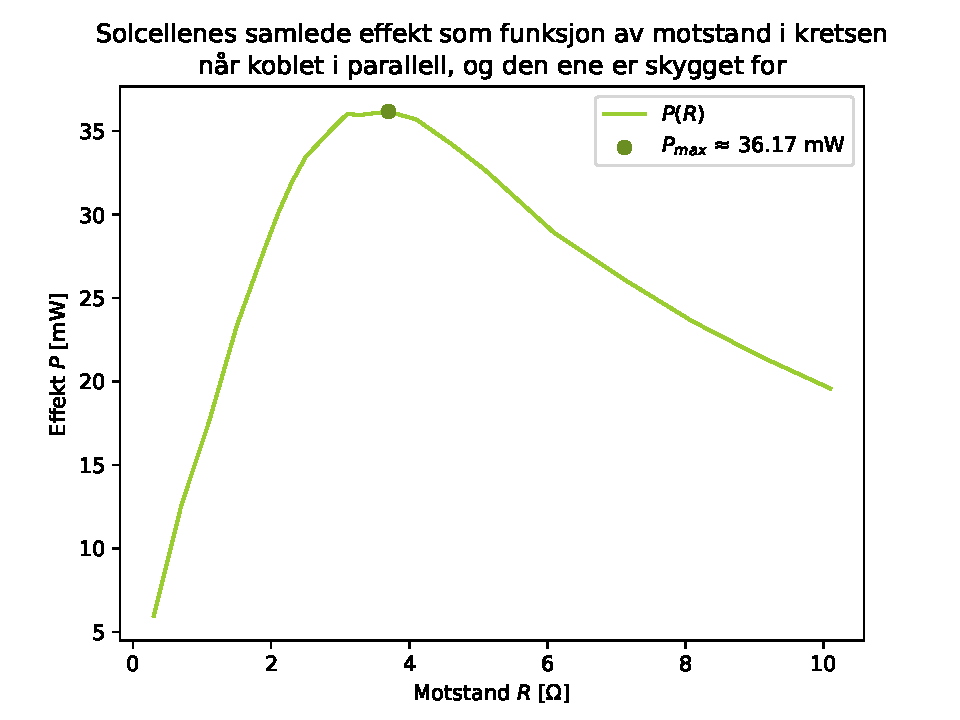
\includegraphics[width = .4\textwidth]{solcellen-oppg-4-parallell.pdf}
  \caption{Solcellens effekt som funksjon av motstand for to solceller koblet i parallel med skygge}
  \label{fig: effekt-motstand-parallell-skygge}
\end{figure}
Vi leser av \cref{fig: effekt-motstand-serie-skygge} som gir oss $R_{opt} = 15.1$ Ohm og $P_{max} = 33.0$ mW for solcellene koblet i serie og \cref{fig: effekt-motstand-parallell-skygge} som gir oss $R_{opt} = 3.7$ Ohm og $P_{max} = 36.1$ mW for solcellene koblet i parallel.

\section{Diskusjon} \label{sec: discussion}
\subsection{Solcellen som halvlederdiode}
Grafen i \cref{fig: strom-spenningskarakteristikk} viser den forventede oppførselen. I mørket er grafen tilsynelatende "skiftet" oppover, i forhold til grafen med lys.

\subsection{Solcellens optimale belastning}
Kurven som vist i \cref{fig: effekt-motstand} har et klart toppunkt rundt $R = 4$ Ohm. Dette er \textit{ikke} som forventet ettersom det ikke stemmer overens med kurven for to solceller i parallel som vist i \cref{fig: effekt-motstand-serie-parallel}. Vi har antagelig gjort en feil under måling, men årsaken er uvisst. Det kan være et hint i at $R_{opt}$ for solcellen alene er dobbelt så stor som for solcellene i parallel.  

\subsection{Kombinasjon av enkeltsolceller til et solcellepanel}
Grafene i \cref{fig: effekt-motstand-serie-parallel} er som forventet. Vi får et skifte i $R_{opt}$. I tillegg ser vi en liten økning av $P_{max}$. Dette stemmer ikke overens med hva vi forventet. Det skulle ikke være en økning i $P_{max}$, men det kan ha kommet av forflytning av solcellene mellom målingene. 

\subsection{Ikke-uniform belysning}
Ved ikke-uniform belysning får vi ca. samme $P_{max}$, med samme feilkilde som i forrige eksperiment, men det største skifte er endringen i $R_{opt}$. Her ser vi en mye klarere forskjell mellom parallel og seriekobling. Uten skygge var differansen på bare ca. 3 Ohm, men her ser vi en differanse på ca. 21 Ohm. Prosentmessig er det likevel ganske lik økning.  

\section{Konklusjon} \label{sec: conclusion}
De to siste eksperimentene viser at man må ta mange hensyn før man bestemmer seg for serie eller parallel, men særlig hvilken motstand som er optimal. Dette vil endre seg avhengig av hvor mye skygge solcellene får. Hvis man har tenkt til å sette opp solcelle panel på enten hytte eller hus, må man selv vurdere hva som lønner seg. Stabiliteten til parallellkoblinger mot den litt simplere og billiger seriekoblingen er også noe å vurdere. Ved parallel kobling kreves det også tykkere kabling ettersom strømmen er større, som også er dyrere. Her er det altså ikke bare et energi aspekt, men også et økonomisk aspekt. En løsning er å koble opp halvparten av solcellene dine i parallell og serie og måle effekten over tid. Da får man en god indikasjon på hva som er optimalt for sin egen unike situasjon. 
\end{document}